\documentclass[hidelinks,12pt]{article}
\usepackage[left=0.25cm,top=1cm,right=0.25cm,bottom=1cm]{geometry}
%\usepackage[landscape]{geometry}
\textwidth = 20cm
\hoffset = -1cm
\usepackage[utf8]{inputenc}
\usepackage[spanish,es-tabla]{babel}
\usepackage[autostyle,spanish=mexican]{csquotes}
\usepackage[tbtags]{amsmath}
\usepackage{nccmath}
\usepackage{amsthm}
\usepackage{amssymb}
\usepackage{mathrsfs}
\usepackage{graphicx}
\usepackage{subfig}
\usepackage{standalone}
\usepackage[outdir=./Imagenes/]{epstopdf}
\usepackage{siunitx}
\usepackage{physics}
\usepackage{color}
\usepackage{float}
\usepackage{hyperref}
\usepackage{multicol}
%\usepackage{milista}
\usepackage{anyfontsize}
\usepackage{anysize}
%\usepackage{enumerate}
\usepackage[shortlabels]{enumitem}
\usepackage{capt-of}
\usepackage{bm}
\usepackage{relsize}
\usepackage{placeins}
\usepackage{empheq}
\usepackage{cancel}
\usepackage{wrapfig}
\usepackage[flushleft]{threeparttable}
\usepackage{makecell}
\usepackage{fancyhdr}
\usepackage{tikz}
\usepackage{bigints}
\usepackage{scalerel}
\usepackage{pgfplots}
\usepackage{pdflscape}
\pgfplotsset{compat=1.16}
\spanishdecimal{.}
\renewcommand{\baselinestretch}{1.5} 
\renewcommand\labelenumii{\theenumi.{\arabic{enumii}})}
\newcommand{\ptilde}[1]{\ensuremath{{#1}^{\prime}}}
\newcommand{\stilde}[1]{\ensuremath{{#1}^{\prime \prime}}}
\newcommand{\ttilde}[1]{\ensuremath{{#1}^{\prime \prime \prime}}}
\newcommand{\ntilde}[2]{\ensuremath{{#1}^{(#2)}}}

\newtheorem{defi}{{\it Definición}}[section]
\newtheorem{teo}{{\it Teorema}}[section]
\newtheorem{ejemplo}{{\it Ejemplo}}[section]
\newtheorem{propiedad}{{\it Propiedad}}[section]
\newtheorem{lema}{{\it Lema}}[section]
\newtheorem{cor}{Corolario}
\newtheorem{ejer}{Ejercicio}[section]

\newlist{milista}{enumerate}{2}
\setlist[milista,1]{label=\arabic*)}
\setlist[milista,2]{label=\arabic{milistai}.\arabic*)}
\newlength{\depthofsumsign}
\setlength{\depthofsumsign}{\depthof{$\sum$}}
\newcommand{\nsum}[1][1.4]{% only for \displaystyle
    \mathop{%
        \raisebox
            {-#1\depthofsumsign+1\depthofsumsign}
            {\scalebox
                {#1}
                {$\displaystyle\sum$}%
            }
    }
}
\def\scaleint#1{\vcenter{\hbox{\scaleto[3ex]{\displaystyle\int}{#1}}}}
\def\bs{\mkern-12mu}


\title{Funciones de Hermite \\ \large {Tema 5 - Funciones especiales} \vspace{-3ex}}
\author{M. en C. Gustavo Contreras Mayén}
\date{ }

\pagestyle{fancy}
\fancyhf{}
\rhead{Curso MAF}
\lhead{\leftmark}
\rfoot{\thepage}
\setlength{\headheight}{16pt}%

\def\changemargin#1#2{\list{}{\rightmargin#2\leftmargin#1}\item[]}
\let\endchangemargin=\endlist 


\begin{document}
\maketitle
\fontsize{14}{14}\selectfont
\tableofcontents
\newpage

%Referencia: Griffiths - Introduction to quantum mechanics. Cap. 2.3

\section{El oscilador armónico.}

Sabemos que el oscilador armónico clásico consiste de una masa $m$ atada a un resorte con una constante $k$, el movimiento que describe la masa, sigue la ley de Hooke:
\begin{align*}
F = - k \, x = m \, \dv[2]{x}{t}
\end{align*}
que tiene por solución (si omitimos la fricción):
\begin{align*}
x(t) = A \, \sin (\omega \, t) + B \, \cos (\omega \, t)
\end{align*}
donde:
\begin{equation}
\omega \equiv \sqrt{\dfrac{k}{m}}
\label{eq:ecuacion_02_041}
\end{equation}
es la frecuencia angular de oscilación. La energía potencial correspondiente es:
\begin{equation}
V(x) = \dfrac{1}{2} \, k \, x^{2}
\label{eq:ecuacion_02_042}
\end{equation}
cuyo trazo es el de una parábola.
\par
De hecho, no existe como tal un oscilador armónico \emph{perfecto}: si estiramos demasiado el resorte, éste se romperá, por lo que la ley de Hooke ya no se cumple una vez que se alcanza este punto.
\par
Podemos considerar que cualquier potencial es \textit{aproximadamente} parabólico en la vecindad de un mínimo local, como se puede ver en la figura (\ref{fig:figura_02_04}):
\begin{figure}[H]
    \centering
    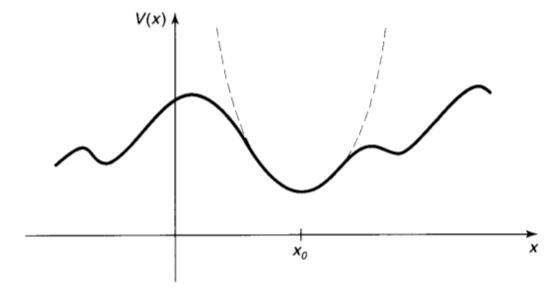
\includegraphics[scale=0.5]{Imagenes/Potencial_arbitrario.png}
    \caption{Aproximación parabólica (curva sesgada) en un potencial arbitrario, en la vecindad de un mínimo local.}
    \label{fig:figura_02_04}
\end{figure}
Es posible expandir el potencial $V(x)$ es una serie de Taylor alrededor del mínimo:
\begin{align*}
V(x) = V(x_{0}) + \pderivada{V} (x_{0}) (x - x_{0}) + \dfrac{1}{2} \sderivada{V} (x_{0}) (x - x_{0}) + \ldots
\end{align*}
Veamos que:
\begin{enumerate}
\item Se puede eliminar $V(x_{0})$, ya que podemos agregar una constante al potencial $V(x)$ y no modifica en nada a la fuerza.
\item Tenemos que $\pderivada{V}(x_{0}) = 0$, ya que $x_{0}$ es un mínimo local.
\item Podemos descartar los términos de orden superior, que se anulan mientras $(x - x_{0})$ se mantenga pequeño.
\end{enumerate}
Por lo que el potencial se representa como:
\begin{align*}
V(x) \cong \dfrac{1}{2} \, \sderivada{V} (x_{0}) (x - x_{0})^{2}
\end{align*}
que describe un oscilación armónica (alrededor de $x_{0}$), con una constante efectiva del resorte $k = \sderivada{V} (x_{0}$).\footnote{Considera que $\sderivada{V}(x_{0})\geq 0$, tomando en cuenta de que $x_{0}$ es un minimo local. En el extraño caso de que $\sderivada{V} (x_{0})= 0$, la oscilación ya no se aproxima a la de un oscilador armónico.}
\par
Esta es la importancia del oscilador armónico: cualquier movimiento oscilatorio se puede aproximar a una oscilación armónica, mientras la amplitud sea pequeña.

\section{El problema del oscilador armónico cuántico.}

El problema cuántico es resolver la ecuación de Schrödinger para el potencial:
\begin{align}
V(x) = \dfrac{1}{2} m \, \omega^{2} \, x^{2}
\label{eq:ecuacion_02_043}
\end{align}
se acostumbra eliminar la constante del resorte para favorecer la frecuencia clásica, usando la ec. (\ref{eq:ecuacion_02_041})
\par
Por lo que basta con resolver la ecuación de Schrödinger independiente del tiempo:
\begin{align}
- \dfrac{\hbar}{2 \, m} \dv[2]{\psi}{x} + \dfrac{1}{2} \, m \, \omega \, x^{2} \, \psi = E \, \psi
\label{eq:ecuacion_02_044}
\end{align}
En la literatura se encontrarán dos enfoques completamente diferentes para resolver este problema.
\begin{enumerate}
\item El primero es una solución de \enquote{fuerza bruta} directa a la ecuación diferencial, que utiliza el método de expansión en una serie de potencias; tiene la virtud de que la misma estrategia se puede aplicar a muchos otros potenciales.
\item El segundo es una técnica algebraica \emph{diabólicamente inteligente}, que utiliza los llamados \textbf{operadores de escalera}.
\end{enumerate}
Primero mostraremos el método algebraico, porque es más rápido y simple (y más divertido).

\subsection{Solución con el método algebraico.}

Antes de iniciar, vamos a escribir la ec. (\ref{eq:ecuacion_02_044}) de una manera más sugestiva:
\begin{align}
\dfrac{1}{2 \, m} \left[ p^{2} + (m \, \omega \, x)^{2} \right] \, \psi = E \, \psi
\label{eq:ecuacion_02_045}
\end{align}
donde:
\begin{align*}
p = \dfrac{\hbar}{i} \dv{x}
\end{align*}
que es el operador momento angular. La idea central es factorizar el Hamiltoniano:
\begin{align}
H = \dfrac{1}{2 \, m} \big[ p^{2} + (m \, \omega \, x)^{2} \big]
\label{eq:ecuacion_02_046}
\end{align}
Si los términos dentro del corchete fueran números, podríamos hacerlo fácilmente, ya que:
\begin{align*}
u^{2} + v^{2} = ( i \, u +  v)(- i \, u + v)
\end{align*}
Pero no es del todo simple, ya que $p$ y $x$ son \textbf{operadores}, y los operadores en general, \textit{no conmutan} ($x \, p$ no es lo mismo que $p \, x$). Aún así, veamos la siguiente expresión:
\begin{align}
a_{\pm} \equiv \dfrac{1}{\sqrt{2 \, \hbar \, m \, \omega }} \left( \mp i \, p + m \, \omega \, x \right)
\label{eq:ecuacion_02_047}
\end{align}
¿Cuál es el producto de $a_{-} \, a_{+}$?
\begin{align*}
a_{-} \, a_{+} &= \dfrac{1}{\sqrt{2 \, \hbar \, m \, \omega }} \left( i \, p + m \, \omega \, x \right) \left( - i \, p + m \, \omega \, x \right) \\[0.5em]
&= \dfrac{1}{\sqrt{2 \, \hbar \, m \, \omega }} \left[ p^{2} + (m \, \omega \, x)^{2} - i \, m \, \omega (x \, p - p \, x) \right]
\end{align*}
Como se anticipó, hay un término adicional que involucra $(x \, p - p \, x)$. A esto lo llamamos \emph{el conmutador} de $x$ y $p$. En general, el conmutador de los operadores\footnote{Revisa las notas complementarias del Tema 3, en donde se repasan los conmutadores y el álgebra de éstos.} $A$ y $B$ (escrito entre corchetes) es:
\begin{align}
[A, B] \equiv A \, B - B \, A
\label{eq:ecuacion_02_048}
\end{align}
Usando esta notación, tenemos que:
\begin{align}
a_{-} \, a_{+} = \dfrac{1}{\sqrt{2 \, \hbar \, m \, \omega }} \big[ p^{2} + (m \, \omega \, x)^{2} \big] - \dfrac{i}{2 \, \hbar} \big[ x , p \big]
\label{eq:ecuacion_02_049}
\end{align}
En donde vemos que se incluye el conmutador de $x$ y $p$. 
\emph{Advertencia}: los operadores pueden ser complicados para trabajar en el concreto con ellos, y estamos obligados a cometer errores a menos que le asignemos una \enquote{función de prueba}, $f (x)$, para que actúen. Al final, podemos deshacernos de la función de prueba y quedaremos con una ecuación que involucra sólo a los operadores. En nuestro caso del oscilador cuántico, tenemos:
\begin{align}
\begin{aligned}[b]
[x, p] \, f(x) &= \left[ x \, \dfrac{\hbar}{i} \, \dv{x} (f) - \dfrac{\hbar}{i} \, \dv{x} (x \, f) \right] = \\[0.5em]
&= \dfrac{\hbar}{i} \left( x \, \dv{f}{x} - x \,\dv{f}{x} - f \right) = \\[0.5em]
&= i \, \hbar \, f(x)
\end{aligned}
\label{eq:ecuacion_02_050}
\end{align}
Haciendo a un lado la función de prueba, tenemos que:
\begin{align}
\setlength{\fboxsep}{3\fboxsep}\boxed{
[x, p] = i \, \hbar
}
\label{eq:ecuacion_02_051}
\end{align}
Este resultado es conocido como la \emph{relación canónica de conmutación}.
\par
Usando esa relación, la ec. (\ref{eq:ecuacion_02_049}) pasa a ser:
\begin{align}
a_{-} \, a_{+} = \dfrac{1}{\hbar \, \omega} \, H + \dfrac{1}{2}
\label{ec:ecuacion_02_052}
\end{align}
o de manera equivalente:
\begin{align}
H = \hbar \, \omega \left( a_{-} \, a_{+} - \dfrac{1}{2} \right)
\label{ec:ecuacion_02_053}
\end{align}
Es claro que el Hamiltoniano no es factorizable de una manera perfecta, ya que hay un término adicional: $(-1/2)$ a la derecha. Es importante resaltar el \emph{orden} de $a_{+}$ y $a_{-}$, con el mismo argumento pero $a_{+}$ a la izquierda, se tiene que:
\begin{align}
a_{+} \, a_{-} = \dfrac{1}{\hbar \, \omega} \, H - \dfrac{1}{2}
\label{eq:ecuacion_02_054}
\end{align}
En particular:
\begin{align}
[a_{-}, a_{+}] = 1
\label{eq:ecuacion_02_55}
\end{align}
El Hamiltoniano se puede escribir como:
\begin{align}
H = \hbar \, \omega \left( a_{+} \, a_{-} +\dfrac{1}{2} \right)
\label{eq:ecuacion_02_056}
\end{align}
En términos de $a_{\pm}$, la ecuación de Schrödinger se puede escribir como:
\begin{align}
\hbar \omega \, \left( a_{\pm} \, a_{\mp} \pm \dfrac{1}{2} \right) \, \psi = E \, \psi
\label{eq:ecuacion_02_057}
\end{align}
Ahora, aquí viene \emph{el paso crucial}: afirmamos que si $\psi$ cumple con la ecuación de Schrödinger, con la energía $E$ (es decir: $H \, \psi = E \, \psi)$, entonces $a_{+} \, \psi$ satisface la ecuación de Schrödinger con la energía $(E + \hbar \, \omega)$:
\begin{align*}
H (a_{+} \, \psi) = (E + \hbar \, \omega)(a_{+} \, \psi)
\end{align*}
Veamos la demostración:
\begin{align*}
H(a_{+} \, \psi) &= \hbar \, \omega \left( a_{+} \, a_{-} + \dfrac{1}{2} \right) (a_{+} \, \psi) = \\[0.5em]
&= \hbar \, \omega \left( a_{+} \, a_{-} \, a_{+} + \dfrac{1}{2} \right) \, \psi = \\[0.5em]
&= \hbar \, \omega \, a_{+} \left( a_{-} \, a_{+} + \dfrac{1}{2} \right) \, \psi = \\[0.5em]
&= a_{+} \left[ \hbar \, \omega \, \left( a_{-} \, a_{+} + 1 -  \dfrac{1}{2}  \right) \right] \\[0.5em]
&= a_{+} \, (H + \hbar \, \omega) \, \psi = \\[0.5em]
&= a_{+} \, (E + \hbar \, \omega) \, \psi =\\[0.5em]
&= (E + \hbar \, \omega)(a_{+} \, \psi) \, \qed
\end{align*}
Obsérvese que mientras que el orden de $a_{+}$ y de $a_{-}$ sí importa, el ordenamiento de $a_{\pm}$ y cualquier constante (como $\hbar$, $\omega$, y $E$) no importa tanto.
\par
De la misma manera, $a_{-} \, \psi$ es una solución con energía $(E - \hbar \, \omega)$:
\begin{align*}
H(a_{-} \, \psi) &= \hbar \, \omega \left( a_{-} \, a_{+} - \dfrac{1}{2} \right) (a_{-} \, \psi) = \\[0.5em]
&= \hbar \, \omega \, a_{-} \, \left( a_{+} \, a_{-} - \dfrac{1}{2} \right) \, \psi = \\[0.5em]
&= a_{-} \left[ \hbar \, \omega \, \left( a_{-} \, a_{+} - 1 -  \dfrac{1}{2}  \right) \right] \\[0.5em]
&= a_{-} \, (H - \hbar \, \omega) \, \psi = \\[0.5em]
&= a_{-} \, (E - \hbar \, \omega) \, \psi =\\[0.5em]
&= (E - \hbar \, \omega)(a_{-} \, \psi) \, \qed
\end{align*}
Entonces, tenemos una máquina maravillosa para extraer nuevas soluciones, con energías más altas y más bajas, ¡si podemos encontrar una solución, para comenzar!
\par
Llamamos a los $a_{\pm}$ \textbf{operadores de escalera}, porque nos permiten subir y bajar en energía:
\begin{itemize}
\item $a_{+}$ se llama operador de ascenso (de subida o de creación).
\item $a_{-}$ se llama operador de descenso (de bajada o de aniquilación).
\end{itemize}
La \enquote{escalera} de estados se ilustra en la figura (\ref{fig:figura_002}).
\begin{figure}[H]
    \centering
    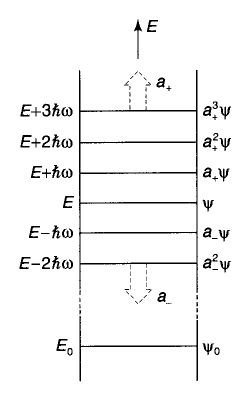
\includegraphics[scale=0.7]{Imagenes/Operadores_escalera.png}
    \caption{Escalera de estados estacionarios para el oscilador armónico.}
    \label{fig:figura_002}
\end{figure}
¡Pero espera! ¿Qué pasa si aplicamos el operador de descenso repetidamente? ¡Eventualmente llegaremos a un estado con una energía menor que cero, que no existe! En algún momento la máquina debe fallar. ¿Cómo puede suceder eso? 
\par
Sabemos que $a_{-} \psi$ es una nueva solución para la ecuación de Schrödinger, pero \emph{no hay garantía de que sea normalizable}, podría ser cero o su integral cuadrada podría ser infinita. Conclusión: Debe presentarse un \enquote{peldaño más bajo} (llamémoslo $\psi_{0}$) tal que:
\begin{align}
a_{-} \, \psi_{0} = 0
\label{eq:ecuacion_02_058}
\end{align}
Usamos esto para determinar $\psi_{0}$:
\begin{align*}
\dfrac{1}{\sqrt{2 \, \hbar \, m \, \omega}} \left( \hbar \, \dv{x} + m \, \omega \, x \right) \, \psi_{0} = 0
\end{align*}
de manera equivalente tenemos que:
\begin{align*}
\dv{\psi_{0}}{x} = - \dfrac{m \, \omega}{\hbar} \, x \, \psi_{0}
\end{align*}
La ED para $\psi_{0}$ es fácil de resolver:
\begin{align*}
\scaleint{6ex} \dv{\psi_{0}}{\psi_{0}} = - \dfrac{m \, \omega}{\hbar} \scaleint{6ex} x \dd{x} \hspace{0.5cm} \Longrightarrow \hspace{0.5cm} \ln \psi_{0} = - \dfrac{m \, \omega}{2 \, \hbar} \, x^{2} + \text{ constante}
\end{align*}
entonces:
\begin{align}
\psi_{0} (x) = A_{0} \, \exp \left( - \dfrac{m \, \omega}{2 \, \hbar} x^{2} \right)
\end{align}
Que podemos normalizar de la siguiente manera:
\begin{align*}
1 = \abs{A}^{2} &= \scaleint{6ex}_{\bs -\infty}^{\infty} \exp \left( - \dfrac{m \, \omega \, x^{2}}{\hbar} \right) \dd{x} = \\[0.5em]
&= \abs{A}^{2} \, \sqrt{\dfrac{\pi \, \hbar}{m \, \omega}}
\end{align*}
tal que $A^{2} = \sqrt{m \, \omega / \pi \, \hbar}$, por lo tanto:
\begin{align}
\setlength{\fboxsep}{3\fboxsep}\boxed{
\psi_{0} = \left( \dfrac{m \, \omega}{\pi \, \hbar} \right)^{1/4} \, \exp \left( - \dfrac{m \, \omega}{2 \, \hbar} \, x^{2} \right)
}
\label{eq:ecuacion_02_059}
\end{align}
Para conocer la energía en este estado, usamos este resultado en la ecuación de Schrödinger (en la forma de la ec. (\ref{eq:ecuacion_02_057})), $\hbar \, \omega \, a_{+} \, a_{-} + (1/2) \, \psi_{0}  = E_{0} \, \psi_{0}$ y aprovechamos el hecho de que $a_{-} \, \psi_{0} = 0$. Por lo que:
\begin{align}
E_{0} = \dfrac{1}{2} \hbar \, \omega
\label{eq:ecuacion_02_060}
\end{align}
Ahora con nuestro pie firmemente plantado en el \enquote{peldaño inferior}\footnote{Toma en cuenta que solo puede haber una escalera, ya que el estado más bajo está determinado únicamente por la ec. (\ref{eq:ecuacion_02_047}). Así, de hecho, se han obtenido todas las soluciones (normalizables).} que es el estado base del oscilador cuántico, simplemente aplicamos el operador de subida para generar los estados excitados\footnote{ En el caso del oscilador armónico, es conveniente apartarse de la costumbre habitual y numerar los estados que comienzan con $n = 0$ en lugar de $n = 1$.}, incrementando la energía en $\hbar \, \omega$ en cada paso:
\begin{align}
\setlength{\fboxsep}{3\fboxsep}\boxed{ \psi_{n} (x) = A_{n} \, (a_{+})^{n} \, \psi_{0} \hspace{1.2cm} \mbox{con } E = \left( n + \dfrac{1}{2} \right) \hbar \, \omega}
\label{eq:ecuacion_02_061}
 \end{align}
donde $A_{n}$ es la constante de normalización. Aplicando el operador de ascenso (repetidamente) a $\psi_{0}$, entonces, podemos (teóricamente) construir todos los estados estacionarios del oscilador armónico. Mientras tanto, sin hacer eso explícitamente, hemos determinado las energías permitidas.
\par
Este método no determina de manera automática la normalización del factor $A_{n}$. Por ejemplo: para determinar el primer estado excitado del oscilador armónico: usamos la ec. (\ref{eq:ecuacion_02_061})
\begin{align}
\begin{aligned}[b]
\psi_{1} &= A_{1} \, a_{+} \, \psi_{0} = \\[1em]
&= A_{1} \, \dfrac{1}{\sqrt{2 \, \hbar \, m \, \omega}} \left( \hbar \, \dv{x} + m \, \omega \, x \right) \, \left( \dfrac{m \, \omega}{\pi \, \hbar} \right)^{1/4} \exp \left( - \dfrac{m \, \omega}{2 \, \hbar} x^{2} \right) = \\[1em]
&= A_{1} \, \left( \dfrac{m \, \omega}{\pi \, \hbar} \right)^{1/4} \sqrt{\dfrac{2 \, m \, \omega}{\hbar}} \, x \, \exp \left( - \dfrac{m \, \omega}{2 \, \hbar} x^{2} \right)
\end{aligned}
\label{eq:ecuacion_02_062}
\end{align}
que podemos normalizar a \enquote{a mano}:
\begin{align*}
\int \abs{\psi_{1}}^{2} \dd{x} &= \abs{A_{1}}^{2} \, \sqrt{ \dfrac{m \, \omega}{\pi \, \hbar}} \, \left( \dfrac{2 \, m \, \omega}{\hbar} \right) \,\int_{-\infty}^{\infty} x^{2} \, \exp \left( - \dfrac{m \, \omega}{\hbar} x^{2} \right) \dd{x} = \\[0.5em]
&= \abs{A_{1}}^{2}
\end{align*}
por tanto: $A_{1} = 1$.
\par
No quisiéramos calcular $\psi_{50}$ de esta manera, pero no importa: hemos encontrado todas las energías permitidas y en principio la ec. (\ref{eq:ecuacion_02_061}) es quien hace el trabajo, excepto la normalización.
\par
Incluso se puede obtener la normalización algebraicamente, pero requiere de un proceso elegante, así que observemos de cerca. Sabemos que $a_{\pm} \, \psi_{n}$ es proporcional $\psi_{n \pm 1}$,
\begin{align}
a_{+} \, \psi_{n} = c_{n} \, \psi_{n+1} \hspace{1cm} a_{-} \, \psi_{n} = d_{n} \, \psi_{n-1}
\label{eq:ecuacion_02_063}
\end{align}
pero ¿cuáles son los factores de proporcionalidad $c_{n}$ y $d_{n}$?.
\par
Veamos primero que para \enquote{cualesquiera} funciones $f(x)$ y $g(x)$
\begin{align}
\scaleint{6ex}_{\bs -\infty}^{\infty} f^{*} \, (a_{\pm} \, g) \dd{x} = \scaleint{6ex}_{\bs -\infty}^{\infty} (a_{\mp} \, f)^{*} \, g \dd{x}
\label{eq:ecuacion_02_064}
\end{align}
Desde el punto de vista del álgebra lineal: $a_{\mp}$ es el \textbf{Hermitiano conjugado} de $a_{\pm}$.
\par
En particular:
\begin{align*}
\scaleint{6ex}_{\bs -\infty}^{\infty} (a_{\pm} \, \psi_{n})^{*} \, (a_{\mp} \, \psi_{n}) \dd{x} = \scaleint{6ex}_{\bs -\infty}^{\infty} (a_{\mp} \, a_{\pm} \, \psi_{n})^{*} \, \psi_{n} \dd{x}
\end{align*}
Al utilizar las ecs. (\ref{eq:ecuacion_02_057}) y (\ref{eq:ecuacion_02_061}), se tiene que:.
\begin{align}
a_{+} \, a_{-} \, \psi_{n} = n \, \psi_{n} \hspace{1.5cm} a_{-} \, a_{+} \, \psi_{n} = (n + 1) \, \psi_{n}
\label{eq:ecuacion_02_065}
\end{align}
así:
\begin{align*}
\scaleint{6ex}_{\bs -\infty}^{\infty} (a_{+} \, \psi_{n})^{*} \, (a_{+} \, \psi_{n}) \dd{x} &= \abs{c_{n}}^{2} \, \scaleint{6ex}_{\bs -\infty}^{\infty} \abs{\psi_{n+1}}^{2} \dd{x} = \\[0.5em]
&= (n + 1) \, \scaleint{6ex}_{\bs -\infty}^{\infty} \abs{\psi_{n}}^{2} \dd{x} 
\end{align*}
y
\begin{align*}
\scaleint{6ex}_{\bs -\infty}^{\infty} (a_{-} \, \psi_{n})^{*} \, (a_{-} \, \psi_{n}) \dd{x} &= \abs{d_{n}}^{2} \, \scaleint{6ex}_{\bs -\infty}^{\infty} \abs{\psi_{n-1}}^{2} \dd{x} = \\[0.5em]
&= n \, \scaleint{6ex}_{\bs -\infty}^{\infty} \abs{\psi_{n}}^{2} \dd{x} 
\end{align*}
Considerando que $\psi_{n}$ y $\psi_{n \pm 1}$ están normalizadas, se tiene entonces que: $\abs{c_{n}}^{2} = n + 1$ y $\abs{d_{n}}^{2} = n$, por lo tanto
\begin{align}
\setlength{\fboxsep}{3\fboxsep}\boxed{
a_{+} \, \psi_{n} = \sqrt{n + 1} \, \psi_{n+1} \hspace{1.5cm} a_{-} \, \psi_{n} = \sqrt{n} \, \psi_{n-1}
}
\label{eq:ecuacion_02_066}
\end{align}
Entonces:
\begin{align*}
\psi_{1} &= a_{+} \, \psi_{0} \\[0.5em]
\psi_{2} &= \dfrac{1}{\sqrt{2}} \, a_{+} \, \psi_{1} = \dfrac{1}{\sqrt{2}} \, (a_{+})^{2} \, \psi_{0} \\[0.5em]
\psi_{3} &= \dfrac{1}{\sqrt{3}} \, a_{+} \, \psi_{2} = \dfrac{1}{\sqrt{3 \cdot 2}} \, (a_{+})^{3} \, \psi_{0} \\[0.5em]
\psi_{4} &= \dfrac{1}{\sqrt{4}} \, a_{+} \, \psi_{3} = \dfrac{1}{\sqrt{4 \cdot 3 \cdot 2}} \, (a_{+})^{4} \, \psi_{0} \\[0.5em]
\vdots
\end{align*}
y así sucesivamente, por lo que:
\begin{align}
\psi_{n} = \dfrac{1}{\sqrt{n!}} \, (a_{+})^{n} \, \psi_{0}
\label{eq:ecuacion_02_067}
\end{align}
lo que quiere decir que el factor de normalización en la ec, \ref{eq:ecuacion_02_061} es $A_{n} = 1 / \sqrt{n!}$  (en particular, $A_{1} = 1$), lo que confirma nuestro resultado.

\subsection{Solución con el método analítico.}

Regresamos nuevamente a la ecuación de Schrödinger para el oscilador armónico:
\begin{align}
- \dfrac{\hbar^{2}}{2 \, m} \, \dv[2]{\psi}{x} + \dfrac{1}{2} \, m \, \omega^{2} \, x^{2} \, \psi = E \, \psi
\label{eq:ecuacion_02_070}
\end{align}
que resolveremos directamente, con el método de series. Para un desarrollo más claro, hacemos el siguiente cambio de variable adimensional:
\begin{align}
\xi \equiv \sqrt{ \dfrac{m \, \omega}{\hbar}} \, x
\label{eq:ecuacion_02_071}
\end{align}
por lo que en términos de $\xi$, la ecuación de Schrödinger toma la forma:
\begin{align}
\dv[2]{\psi}{\xi} = (\xi^{2} - K) \, \psi
\label{eq:ecuacion_02_072}
\end{align}
donde $K$ es la energía, en unidades de $(1/2) \, \hbar \, \omega$:
\begin{align}
K \equiv \dfrac{2 \, E}{\hbar \, \omega}
\label{eq:ecuacion_02_073}
\end{align}
Nuestro problema es resolver la ec. (\ref{eq:ecuacion_02_072}), y durante el proceso obtener los valores \enquote{permitidos} de $K$ (y por tanto de $E$).
\par
Para iniciar, veamos que para valores muy grandes de $\xi$ (que a la vez, es decir que tendríamos valores muy grandes de $x$), el término $\xi^{2}$ domina sobre la constante $K$, por lo que tendríamos:
\begin{align}
\dv[2]{\psi}{\xi} \approx \xi^{2} \, \psi
\label{eq:ecuacion_02_074}
\end{align}
que tiene por solución:
\begin{align}
\psi (\xi) \approx A \, \exp \left( - \dfrac{\xi^{2}}{2} \right) + B \, \exp \left( + \dfrac{\xi^{2}}{2} \right)
\label{eq:ecuacion_02_075}
\end{align}
en donde encontramos que el término $B$ no se puede normalizar (no funciona cuando $\abs{x} \to \infty$), por lo que las soluciones aceptables con sentido físico, tienen las forma asintótica:
\begin{align}
\psi (\xi) = ( \quad ) \exp \left( - \dfrac{\xi^{2}}{2} \right) \hspace{1.5cm} \text{con valores grandes de } \xi
\label{eq:ecuacion_02_076}
\end{align}
Esto sugiere que \enquote{aprovechamos} la parte exponencial:
\begin{align}
\psi (\xi) = h (\xi) \, \exp \left( - \dfrac{\xi^{2}}{2} \right)
\label{eq:ecuacion_02_077}
\end{align}
esperando que lo que queda de $h (\xi)$ tenga una forma funcional más simple que $\psi (\xi)$ mismo.\footnote{Toma en cuenta que aunque invocamos algunas aproximaciones para motivar la ec. (\ref{eq:ecuacion_02_077}), lo que sigue es exacto. La técnica para eliminar el comportamiento asintótico es el primer paso estándar en el método de la serie de potencias para resolver ecuaciones diferenciales}
\par
Diferenciando la ec. (\ref{eq:ecuacion_02_077}), se tiene que:
\begin{align*}
\dv{\psi}{xi} = \left( \dv{h}{\xi} - \xi \, h \right) \, \exp \left( - \dfrac{\xi^{2}}{2} \right)
\end{align*}
y
\begin{align*}
\dv[2]{\psi}{xi} = \left( \dv[2]{h}{\xi} - 2  \,  \xi \, \, \dv{h}{\xi} + (\xi^{2} - 1) \, h \right) \, \exp \left( - \dfrac{\xi^{2}}{2} \right)
\end{align*}
por lo que la ec. de Schrödinger (ec. \ref{eq:ecuacion_02_072}) es:
\begin{align}
\dv[2]{h}{xi} - 2 \, \xi \, \dv{h}{\xi} +  (K - 1) \, h = 0
\label{eq:ecuacion_02_078}
\end{align}
Proponemos una solución a la ED (\ref{eq:ecuacion_02_078}) en la forma de una serie de potencias en $\xi$ con el método de Frobenius:
\begin{align}
h (\xi) = a_{0} + a_{1} \, \xi + a_{2} \, \xi^{2} + \ldots = \sum_{j=0}^{\infty} a_{j} \, \xi^{j}
\label{eq:ecuacion_02_079}
\end{align}
Diferenciamos en dos ocasiones la solución para obtener:
\begin{align*}
\dv{h}{\xi} &= \sum_{j=0}^{\infty} j \, a_{j} \, \xi^{j-1} \\[0.5em]
\dv[2]{h}{\xi} &= \sum_{j=0}^{\infty} (j + 1)(j + 2) \, a_{j+2} \, \xi^{j}
\end{align*}
que al sustituir en la ec. (\ref{eq:ecuacion_02_078}), tenemos que:
\begin{align}
\sum_{j=0}^{\infty} [ (j + 1)(j + 2) \, a_{j+2} - 2 \, j \, a_{j} +  (K - 1) \, a_{j} ] \, \xi^{j} = 0
\label{eq:ecuacion_02_80}
\end{align}
Sabemos que los coeficientes para cada potencia de $\xi$ deben de anularse, por tanto:
\begin{align*}
(j + 1)(j + 2) \, a_{j+2} - 2 \, j \, a_{j} +  (K - 1) \, a_{j} = 0
\end{align*}
de donde se obtiene que:
\begin{align}
a_{j+2} = \dfrac{(2 \, j + 1 - K)}{(j + 1)(j + 2)} \, a_{j}
\label{eq:ecuacion_02_081}
\end{align}
Esta es la \textbf{fórmula de recursión}, que es, en sí misma, equivalente a la ecuación de Schrödinger. Dado $a_{0}$, podemos obtener todos los coeficientes pares:
\begin{align*}
a_{2} = \dfrac{(1 - K)}{2} \, a_{0} \hspace{1cm} a_{4} = \dfrac{(5 - K)}{12} \, a_{2} = \dfrac{(5 - K)(1 - K)}{24} \, a_{0} \ldots
\end{align*}
comenzando con un $a_{1}$ dado, podemos obtener los coeficientes impares:
\begin{align*}
a_{3} = \dfrac{(3 - K)}{6} \, a_{1} \hspace{1cm} a_{5} = \dfrac{(7 - K)}{20} \, a_{3} = \dfrac{(7 - K)(3 - K)}{120} \, a_{1} \ldots
\end{align*}
\par
Podemos escribir la solución completa:
\begin{align}
h (\xi) = h_{\text{par}} (\xi) + h_{\text{impar}} (\xi)
\label{eq:ecuacion_02_082}
\end{align}
donde:
\begin{align*}
h_{\text{par}} (\xi) = a_{0} + a_{2} \, \xi^{2} + a_{4} \, \xi^{4} + \ldots
\end{align*}
si es una función par de $\xi$ (ya que involucra sólo potencias pares) a partir de $a_{0}$, y como:
\begin{align*}
h_{\text{impar}} (\xi) = a_{1} \, \xi + a_{3} \, \xi^{3} + a_{5} \, \xi^{5} + \ldots
\end{align*}
si es función impar, a partir de $a_{1}$. Entonces tenemos que la ec. (\ref{eq:ecuacion_02_081}) determina a $h(\xi)$ en términos de dos constantes arbitrarias ($a_{0}$ y $a_{1}$), que es lo que se esperaba, dado que tenemos una ED2.
\par
Aún así, no todas las soluciones que se obtienen son normalizables. Para valores grandes de $j$, la fórmula de recursión pasa a ser (aproximadamente):
\begin{align*}
a_{j+2} \approx \dfrac{2}{j} \, a_{j}
\end{align*}
con una solución (aproximada):
\begin{align*}
a_{j} \approx \dfrac{C}{(j/2)!}
\end{align*}
para alguna constante $C$, y esto nos lleva a (para valores grandes de $\xi$, donde las potencias elevadas dominan):
\begin{align*}
h (\xi) \approx C \, \sum \dfrac{1}{(j/2)!} \, \xi^{j} \approx C \, \sum \dfrac{1}{j!} \xi^{2 j} \approx C \, \exp \left( \xi^{2} \right)
\end{align*}
Veamos ahora lo siguiente: si $h \to \exp \left( \xi^{2} \right)$, entonces ¿$\psi \to \exp \left( \xi^{2}/2 \right)$?, por que presenta un comportamiento asintótico que no se desea!
\par
Solo hay una forma de salir de esto: para soluciones normalizables, \textit{la serie de potencias debe terminar}. Debe de presentarse un valor \enquote{mayor} de $j$ (llámalo $n$) de manera que la fórmula de recursión devuelva un $a_{n+2} = 0$ (esto truncará cada una de las series par o impar; la otra debe ser cero desde el principio). Para soluciones físicamente aceptables, entonces, debemos tener que:
\begin{align*}
K = 2 \, n + 1
\end{align*}
para un entero positivo $n$, es decir (refiriéndose a la ecuación (\ref{eq:ecuacion_02_073})) que la energía debe ser de la forma:
\begin{align}
E_{n} = \left( n + \dfrac{1}{2} \right) \, \hbar \, \omega , \hspace{1.5cm} n = 0, 1, 2, \ldots
\label{eq:ecuacion_02_083}
\end{align}
Así recuperamos, mediante un método completamente diferente, la condición fundamental de cuantificación que encontramos algebraicamente en la ec. (\ref{eq:ecuacion_02_061}).
\par
Al principio parece ser bastante sorprendente que la cuantificación de la energía surja de un detalle técnico en la solución de la serie de potencias de la ecuación de Schrodinger, pero veámoslo desde una perspectiva diferente. La ec. (\ref{eq:ecuacion_02_070}) tiene soluciones, por supuesto, para cualquier valor de $E$ (de hecho, tiene dos soluciones linealmente independientes para cada $E$). Pero casi todas estas soluciones no funcionan para $x$ grandes y, por lo tanto, no son normalizables.
\par
Para los valores permitidos de $K$, la fórmula de recursión es:
\begin{align}
a_{j+2} = \dfrac{- 2 (n - j)}{(j + 1)(j + 2)} \, a_{j}
\label{eq:ecuacion_02_084}
\end{align}
Si $n = 0$, hay sólo un término en la serie (debemos de escoger $a_{1} = 0$ para cancelar $h_{\text{impar}}$ y $j = 0$ en la ec. (\ref{eq:ecuacion_02_084}), nos lleva a $a_{2} = 0$):
\begin{align*}
h_{0} (\xi) = a{0}
\end{align*}
y por lo tanto:
\begin{align*}
\psi_{0} (\xi) = a_{0} \, \exp \left( - \dfrac{\xi^{2}}{2} \right)
\end{align*}
que fuera de la normalización, es la ec. (\ref{eq:ecuacion_02_059}).
\par
Para $n=1$, escogemos $a_{0} = 0$ y la ec. (\ref{eq:ecuacion_02_084}) con $j = 1$, nos devuelve $a_{3} = 0$, así:
\begin{align*}
h_{1} (\xi) = a_{1} \, \xi
\end{align*}
por lo que:
\begin{align*}
\psi_{1} (\xi) = a_{1} \, \xi \, \exp \left( - \dfrac{\xi^{2}}{2} \right)
\end{align*}
que confirma la ec. (\ref{eq:ecuacion_02_062}).
\par
Para $n = 2$, $j = 0$, tenemos que $a_{2} = - 2 \, a_{0}$ y $j = 2$ nos da que $a_{4} = 0$ por lo tanto:
\begin{align*}
h_{2} (\xi) = a_{0} (1 - 2 \, \xi^{2})
\end{align*}
y entonces:
\begin{align*}
\psi_{2} (\xi) = a_{0} (1 - 2 \, \xi^{2}) \, \exp \left( - \dfrac{\xi^{2}}{2} \right)
\end{align*}
y así sucesivamente.
\par
En general, $h_{n} (\xi)$ será un polinomio de grado $n$ en $\xi$, que involucra sólo las potencias pares, si $n$ es un entero par, y las potencias impares solamente, si $n$ es un entero impar. Aparte del factor global $(a_{0}$ o $a_{1})$, se tienen los llamados \textbf{polinomios de Hermite}, $H_{n} (\xi)$.
\par
Los primeros polinomios de Hermite se muestran en la tabla (\ref{tabla_001}). 
\begin{center}
\begin{table}[H]
\large
\centering
\begin{tabular}{l l}
$H_{0}(\xi) =$ & $1$ \\
$H_{1}(\xi) =$ & $2 \, \xi$ \\
$H_{2}(\xi) =$ & $4 \, \xi^{2} - 2 $ \\
$H_{3}(\xi) =$ & $8 \, \xi^{3} - 12 \, \xi$ \\
$H_{4}(\xi) =$ & $16 \, \xi^{4} - 48 \, \xi^{2} + 12 $ \\
$H_{5}(\xi) =$ & $32 \, \xi^{5} - 160 \, \xi^{3} + 120 \, \xi$
\end{tabular}
\caption{Primeros polinomios de Hermite $H_{n}(x)$.}
\label{tabla_001}
\end{table}
\begin{figure}[H]
    \centering
    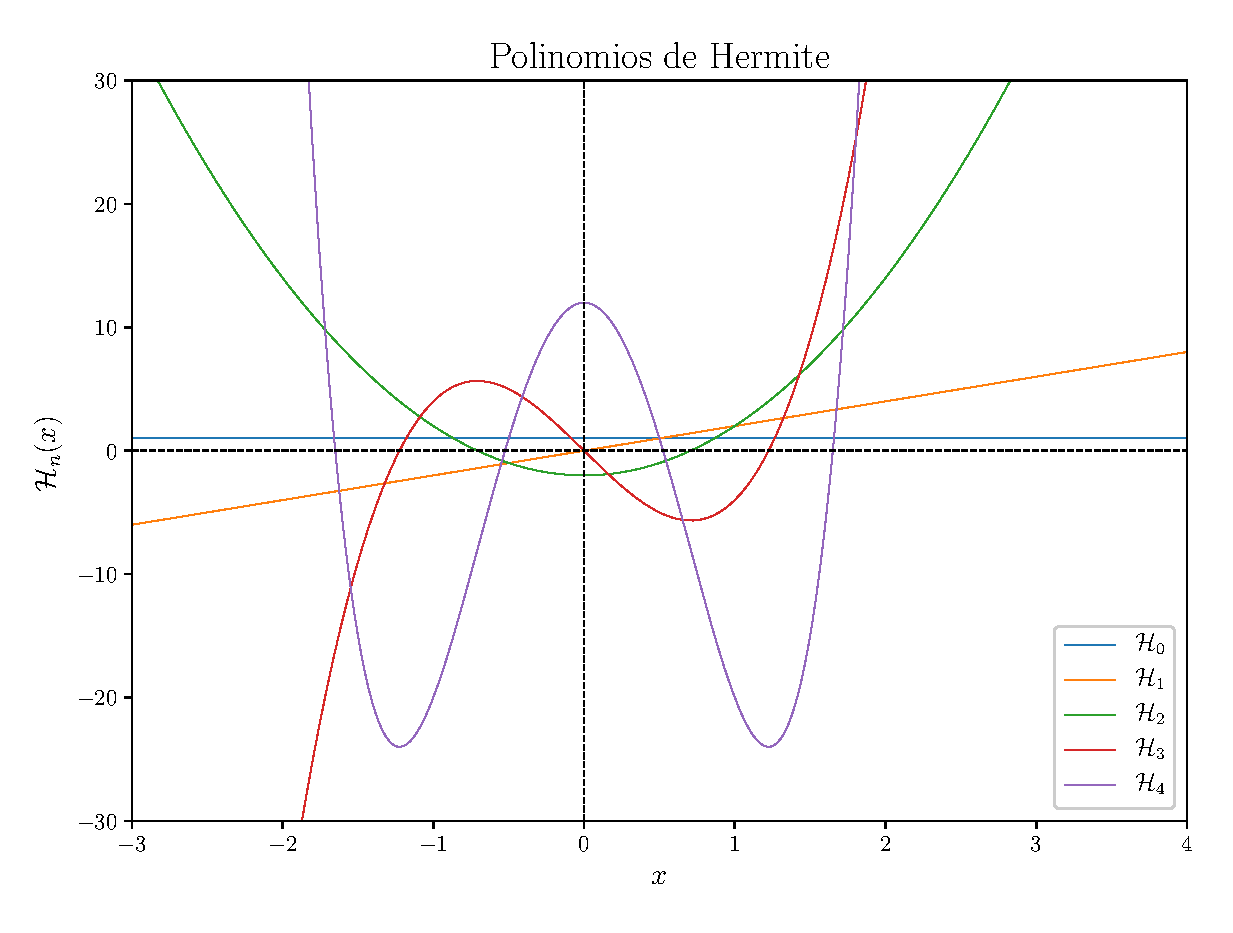
\includegraphics[scale=0.7]{Imagenes/Polinomios_Hermite_01.eps}
    \caption{Gráfica de los primeros polinomios de Hermite.}
    \label{figura_003}
\end{figure}
\end{center}
Por tradición, el factor multiplicativo arbitrario se elige de modo que el coeficiente de la potencia más alta de $\xi$ es $2^{n}$. Con esta convención, los estados estacionarios normalizados para el oscilador armónico son
\begin{align}
\setlength{\fboxsep}{3\fboxsep}\boxed{
\psi_{n} (x) = \left( \dfrac{m \, \omega}{\pi \, \hbar} \right)^{1/4} \, \dfrac{1}{\sqrt{2^{n} \, n!}} \, H_{n} (\xi) \, \exp \left( - \dfrac{\xi^{2}}{2} \right)}
\label{eq:ecuacion_02_069}
\end{align}
Son idénticos (por supuesto) a los que obtuvimos algebraicamente en la ec. (\ref{eq:ecuacion_02_067}).
\newpage
En las siguientes figuras\footnote{La programación se hizo con \texttt{python}, ocupando las librerías de graficación \texttt{matplotlib} y \texttt{scipy} para resolver la ecuación diferencial.}, se han trazado la función $\psi_{n} (x)$ para las primeras $n$'s y su normalización.
\begin{figure}[H]
    \centering
    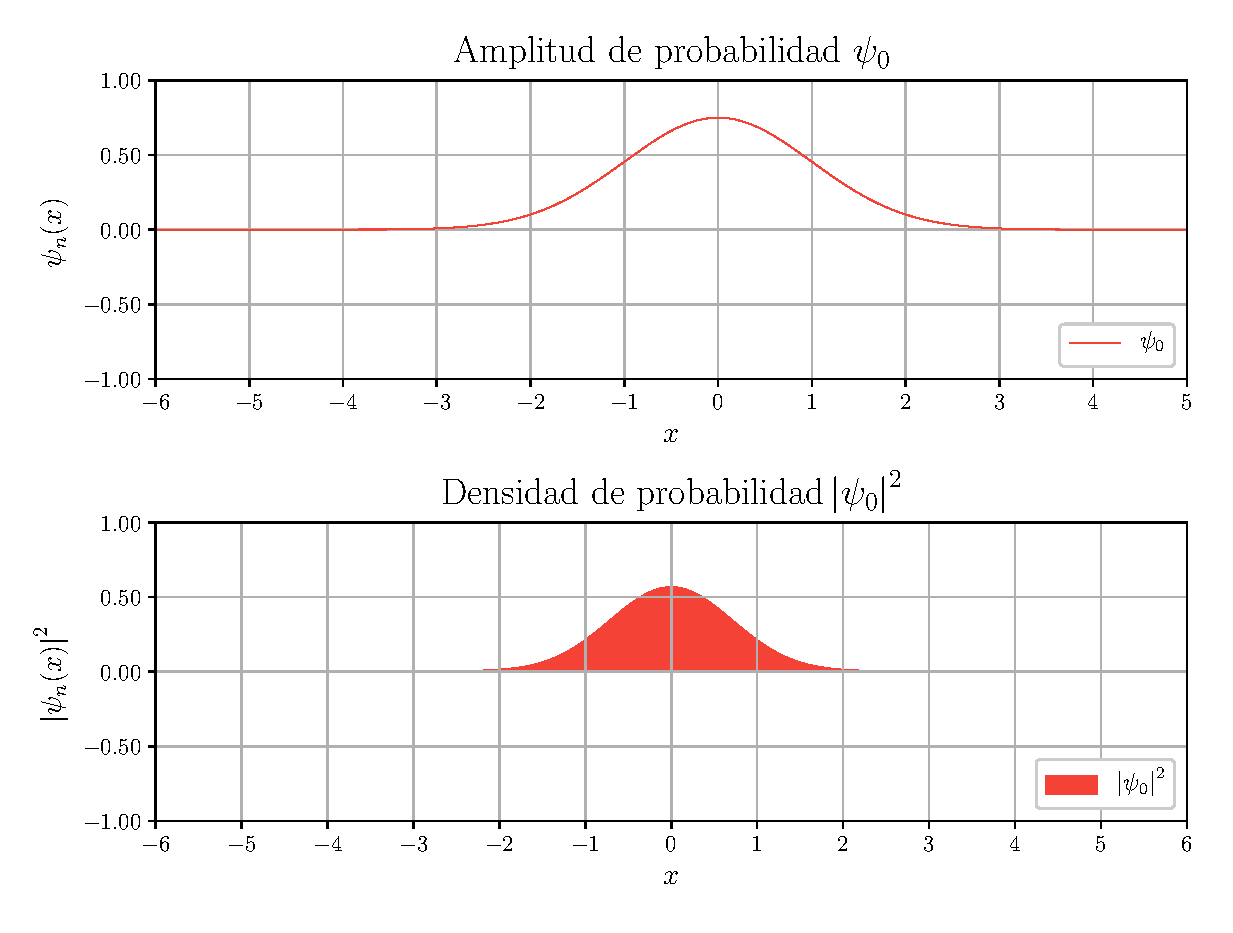
\includegraphics[scale=0.6]{Imagenes/Funcion_Onda_00.eps}
    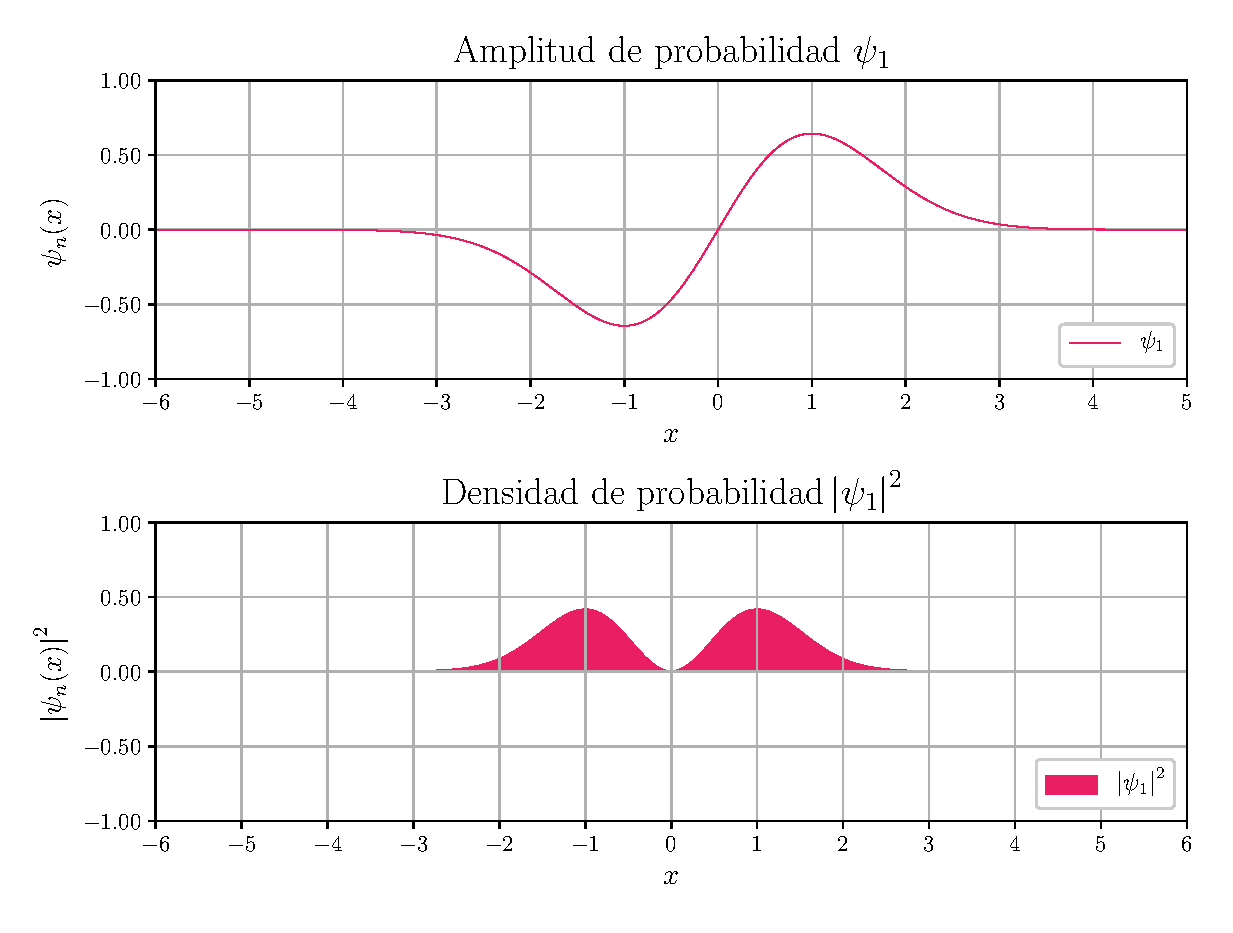
\includegraphics[scale=0.6]{Imagenes/Funcion_Onda_01.eps}
\end{figure}
\begin{figure}[H]
    \centering
    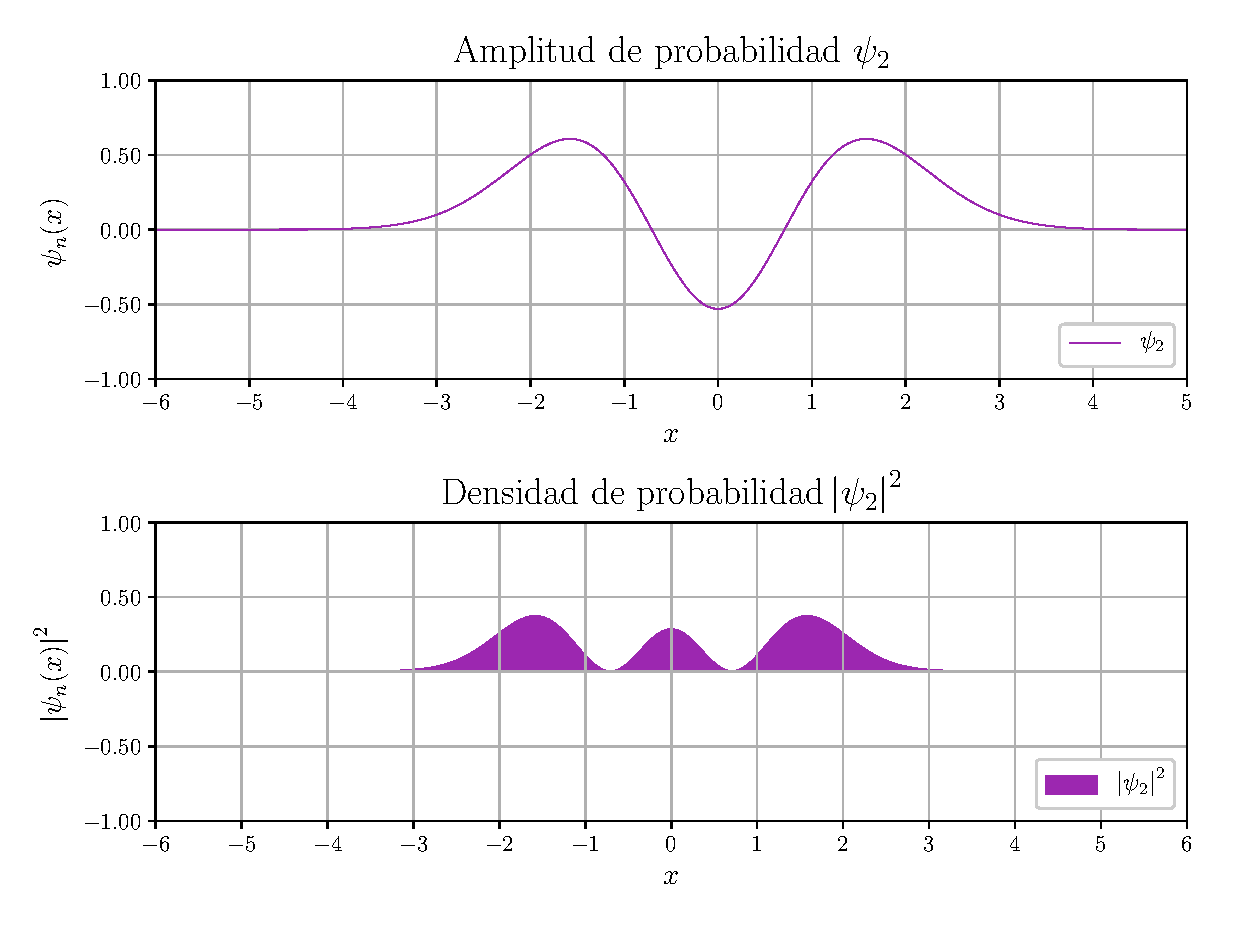
\includegraphics[scale=0.6]{Imagenes/Funcion_Onda_02.eps}
    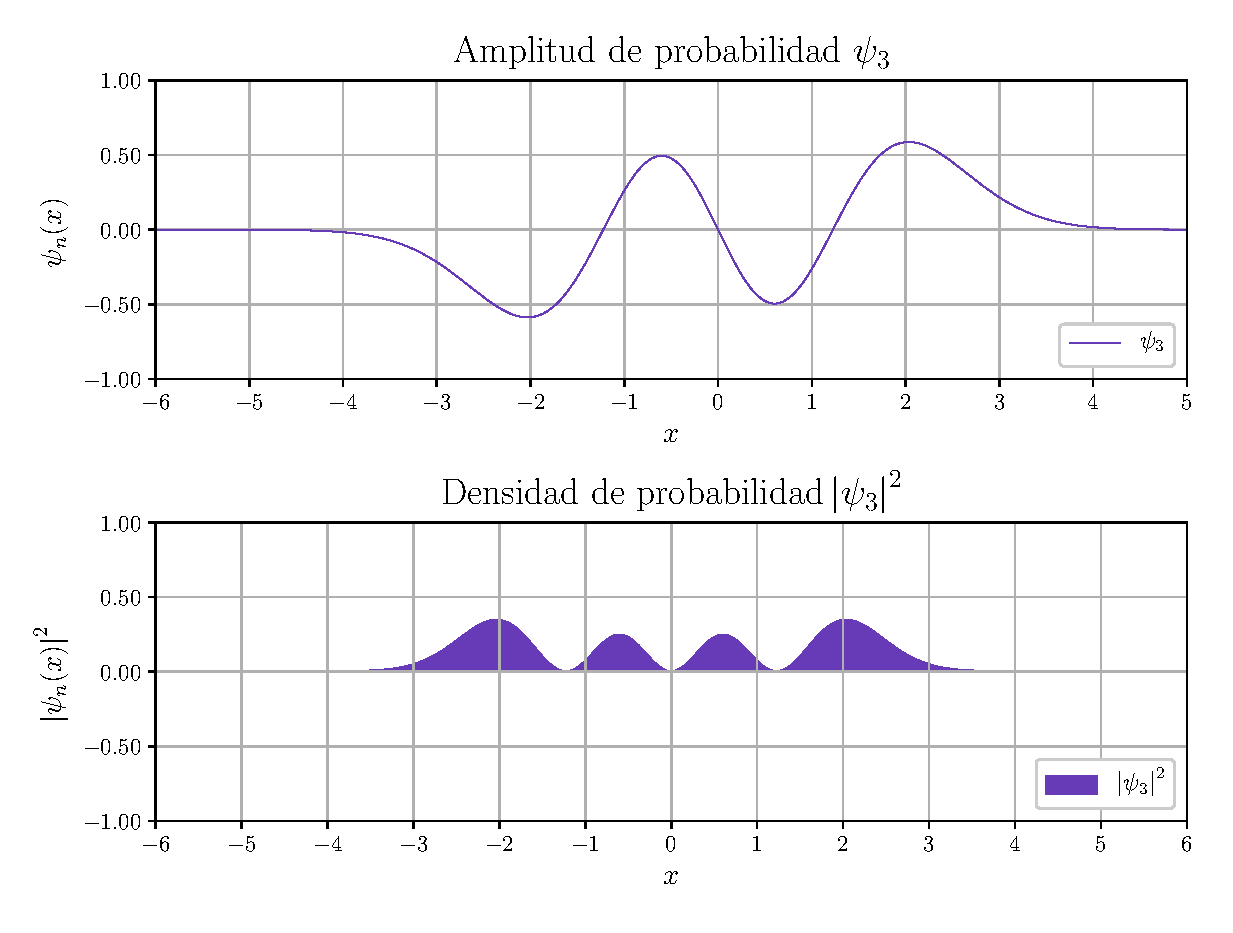
\includegraphics[scale=0.6]{Imagenes/Funcion_Onda_03.eps}
\end{figure}
\begin{figure}[H]
    \centering
    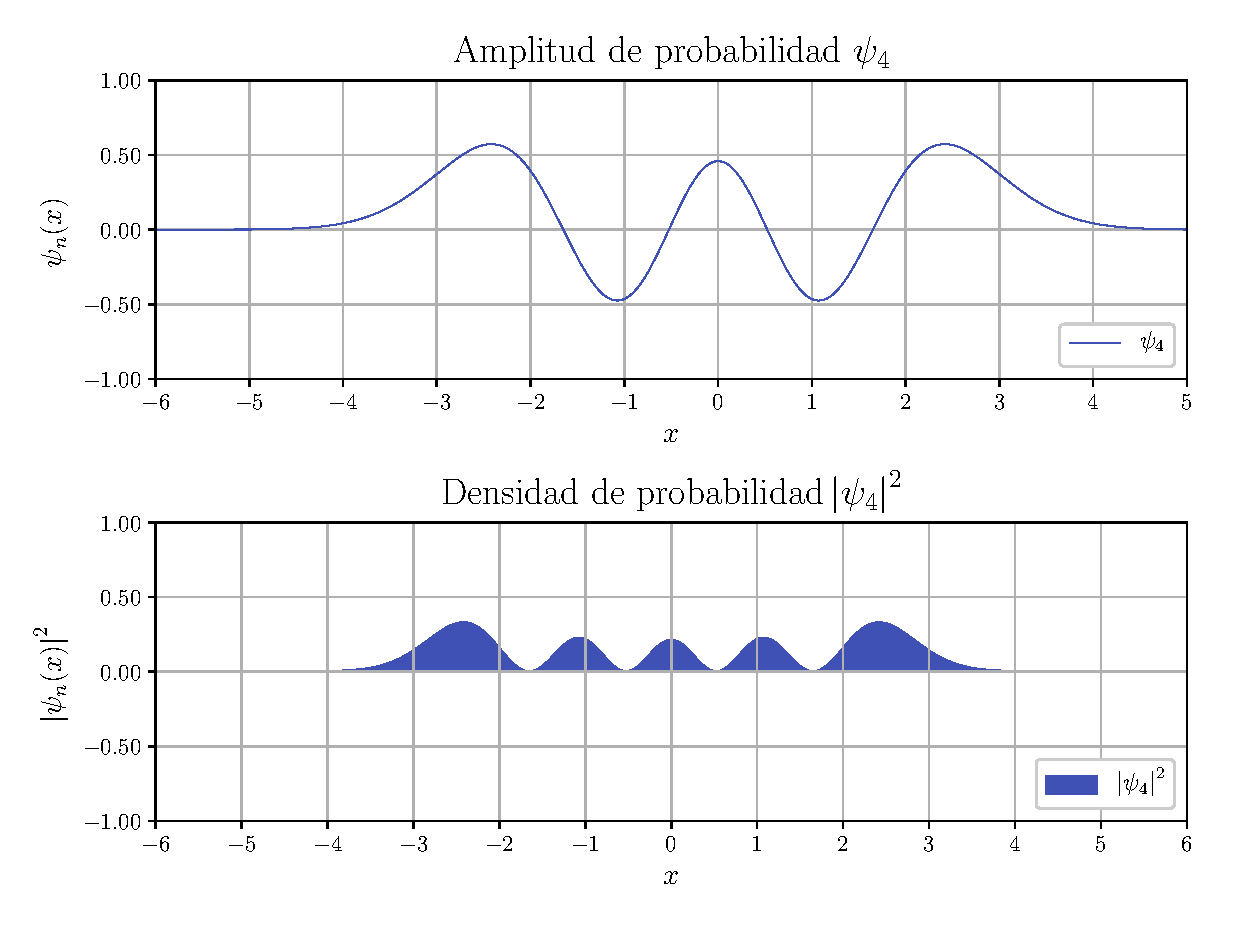
\includegraphics[scale=0.6]{Imagenes/Funcion_Onda_04.eps}
    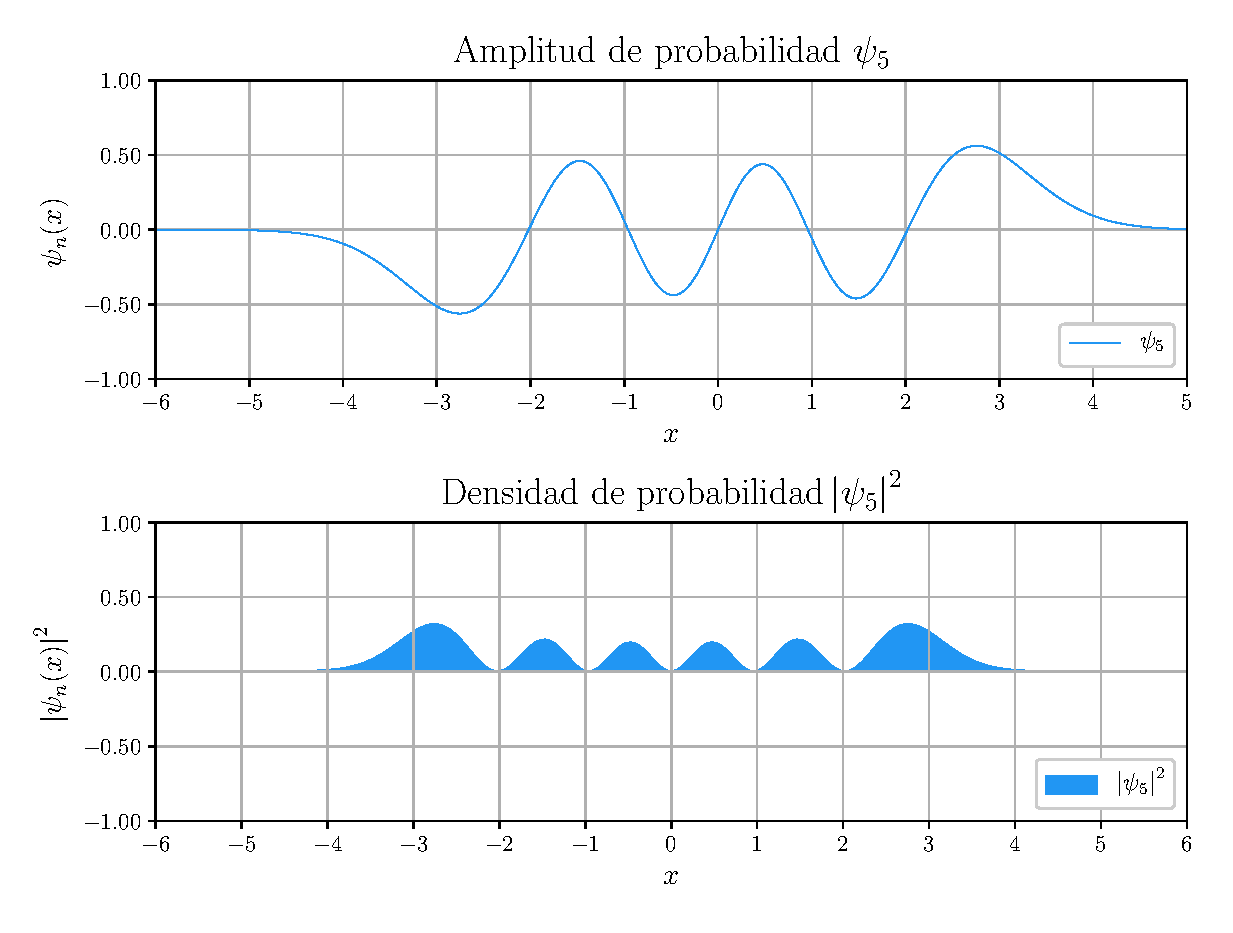
\includegraphics[scale=0.6]{Imagenes/Funcion_Onda_05.eps}
\end{figure}
\begin{figure}[H]
    \centering
    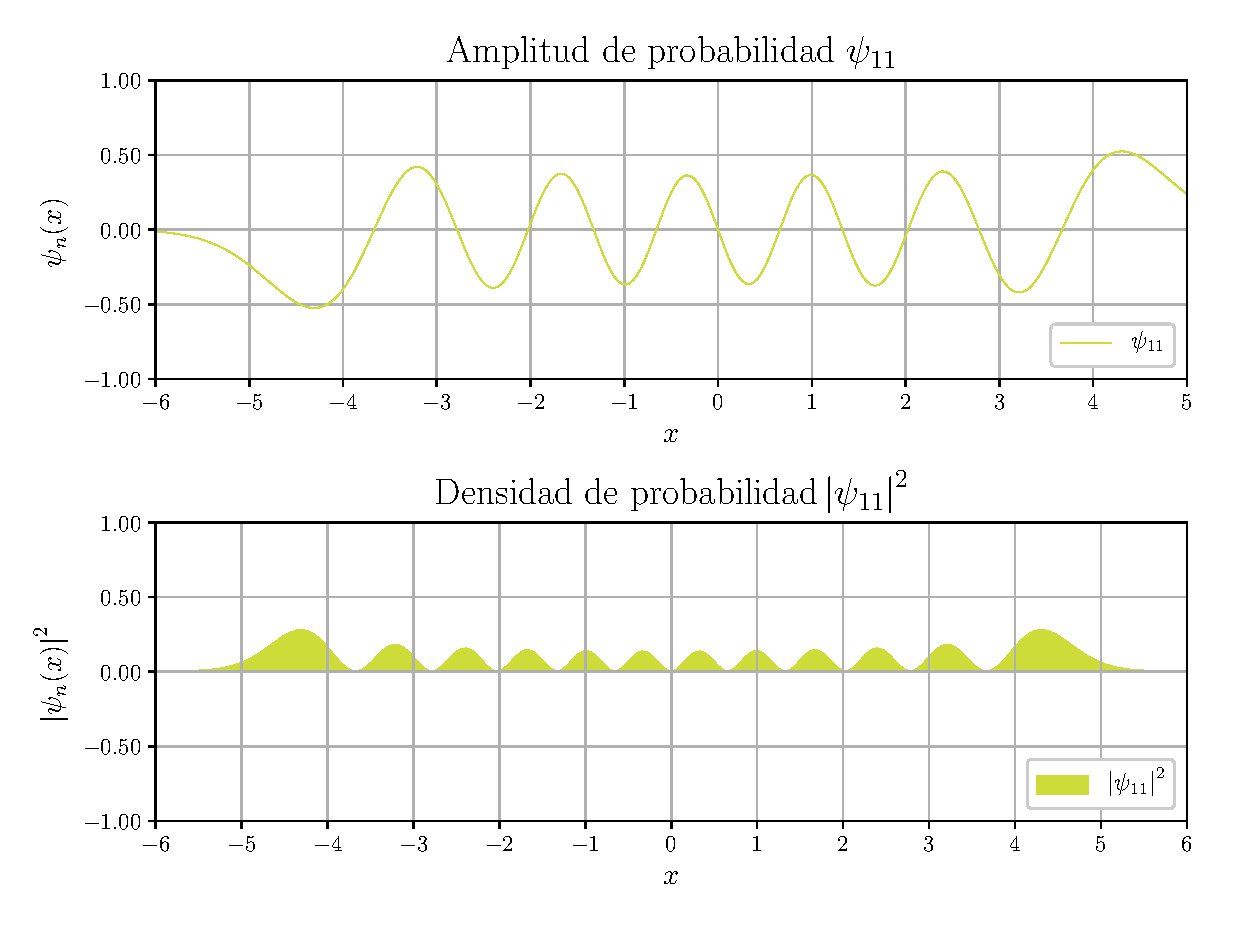
\includegraphics[scale=0.6]{Imagenes/Funcion_Onda_011.eps}
    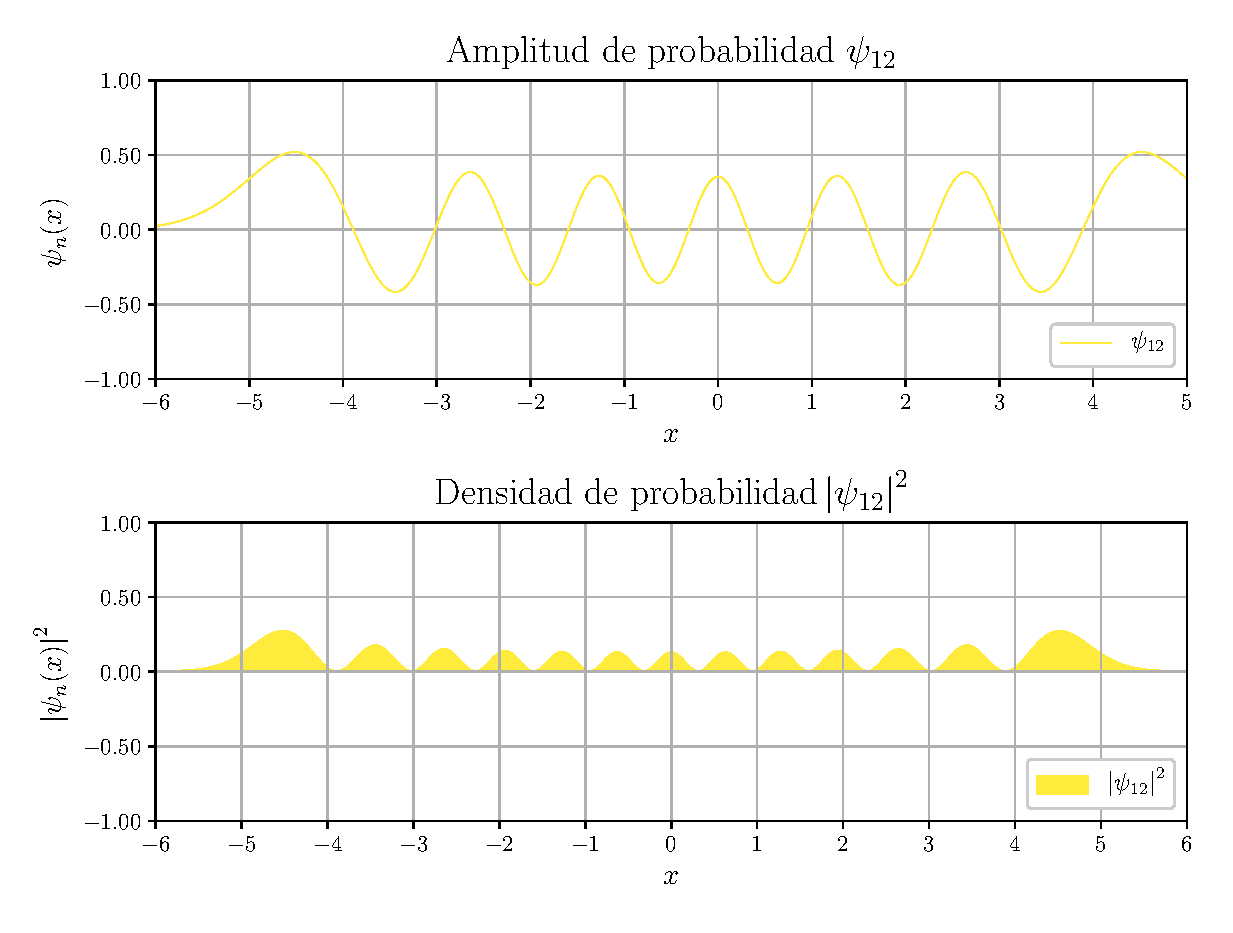
\includegraphics[scale=0.6]{Imagenes/Funcion_Onda_012.eps}
\end{figure}
\newpage
En la siguiente gráfica se han superpuesto el potencial parabólico y las funciones de onda normalizadas, esquemáticamente representa la solución a la ecuación de Schrödinger.
\begin{figure}[H]
    \centering
    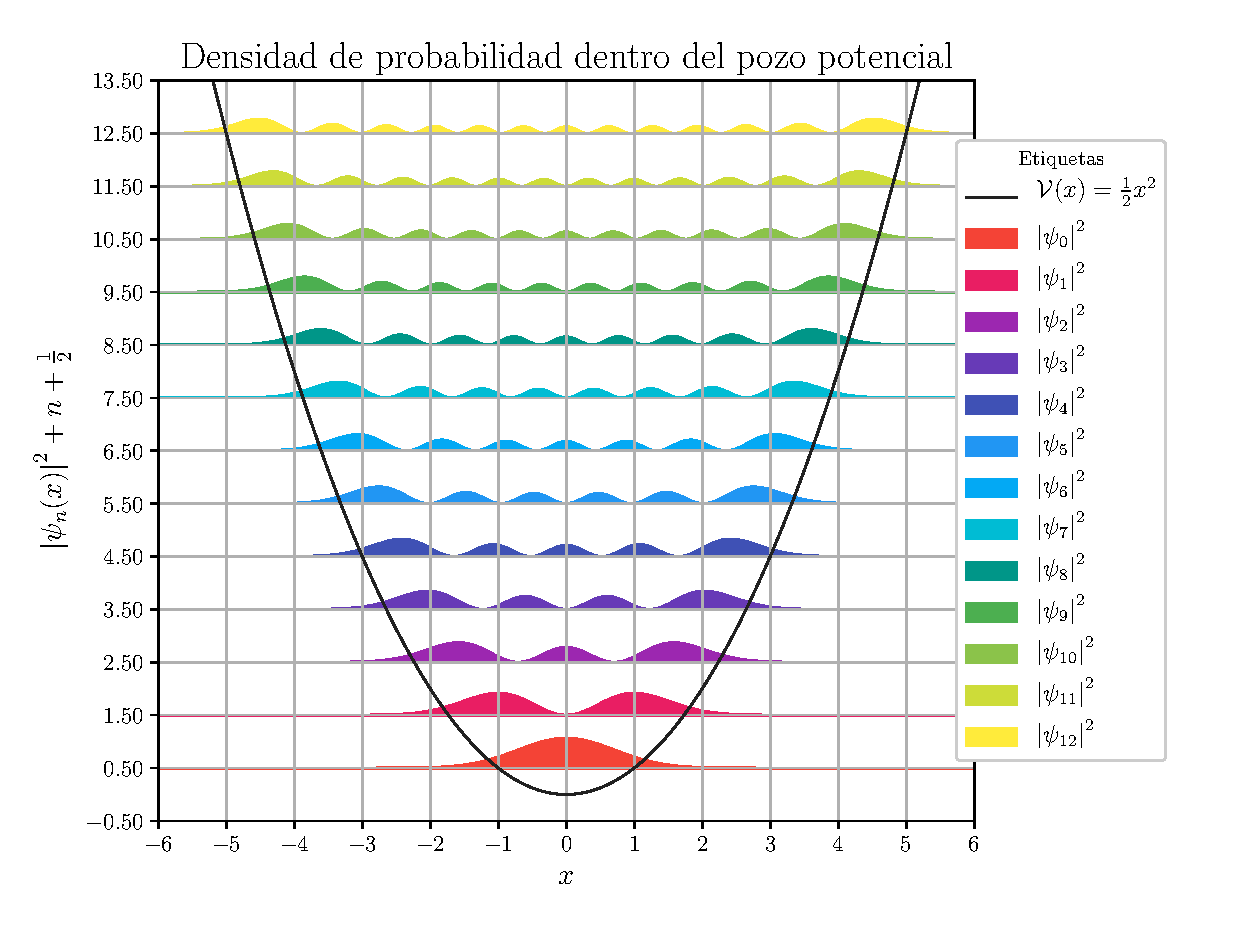
\includegraphics[scale=0.75]{Imagenes/Funciones_Normalizadas_01.eps}
\end{figure}
\newpage
El oscilador cuántico es sorprendentemente diferente de su contraparte clásica: no solo se cuantifican las energías, sino que las distribuciones de posición tienen algunas características extrañas. 
\par
Por ejemplo, la probabilidad de encontrar la partícula fuera del rango permitido clásicamente (es decir, con $x$ mayor que la amplitud clásica para la energía en cuestión) no es cero, y en todos los estados impares la probabilidad de encontrar la partícula en el centro del pozo de potencial es cero. Sólo para valores relativamente grandes de $n$ empezamos a ver alguna semejanza con el caso clásico. 
\begin{figure}[H]
    \centering
    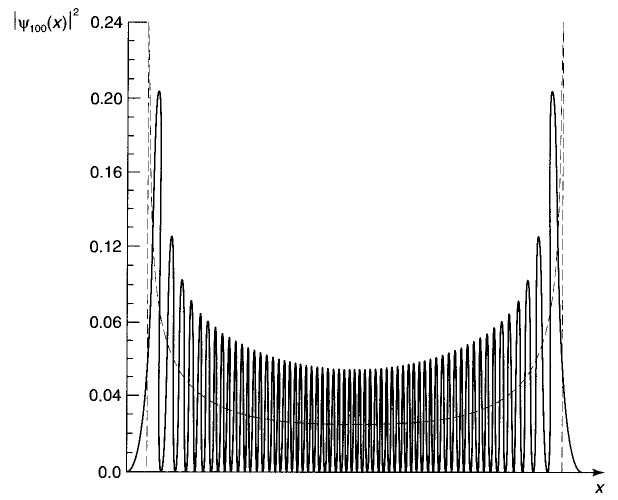
\includegraphics[scale=0.5]{Imagenes/Funcion_Onda_100.png}
    \caption{Gráfica para la función de onda $\abs{\psi_{100}}^{2}$, junto con una distribución clásica (línea punteada).}
    \label{figura_004}
\end{figure}
En la figura (\ref{figura_004}), se han superpuesto la distribución de posición clásica en la cuántica (para $n = 100$); si aplanaramos los bultos, los dos encajarían bastante bien (sin embargo, en el caso clásico estamos hablando de la distribución de posiciones en el tiempo para un oscilador, mientras que en el caso cuántico estamos hablando de la distribución en un conjunto de sistemas preparados de manera idéntica).

%Ref. Riley 18.9 Hermite functions
\section{Propiedades de los Polinomios de Hermite.}
\subsection{Ecuación diferencial.}

La ecuación diferencial de Hermite tiene la forma:
\begin{align}
\sderivada{y} -  2 \, x \, \pderivada{y} + 2 \, \nu \, y = 0
\label{eq:ecuacion_18_126}
\end{align}
y tiene una singularidad esencial en $x = \infty$. El parámetro $\nu$ es un número real dado, aunque casi siempre toma un valor entero en aplicaciones físicas Cualquier solución de la ec. (\ref{eq:ecuacion_18_126}) se llama \emph{función de Hermite}.
\par
En la sección anterior se revisó el desarrollo para la solución con el método de Frobenius, encontrando que:
\begin{align}
H_{n}(x) = \sum_{m=0}^{[n/2]} (-1)^{m} \, \dfrac{n!}{m! \, (n - 2 \, m)!} \, (2 \, x)^{n-2m}
\label{eq:ecuacion_18_129}
\end{align}
donde los $H_{n}(x)$ son llamados los \emph{polinomios de Hermite de orden n}, la notación $[n/2]$ indica la parte entera de $n/2$. Veamos en particular que $H_{n}(-x) = (-1)^{n} \, H_{n}(x)$.

\subsection{Fórmula de Rodrigues.}

La fórmula de Rodrigues para los polinomios de Hermite están dados por:
\begin{align}
H_{n}(x) = (-1)^{n} \, e^{x^{2}} \, \dv[n]{x} \big( e^{-x^{2}} \big)
\label{eq:ecuacion_18_130}
\end{align}
Que se puede demostrar usando el teorema de Leibniz.

\subsection{Ortogonalidad mutua.}

La ecuación de Hermite se puede presentar de la forma Sturm Liouville con $p = \exp(-x^{2})$, $q = 0$, $\lambda = 2 \, n$ y $\rho = \exp(-x^{2})$, por lo que su intervalo natural es $[-\infty, \infty]$.
\par
Dado que los polinomios de Hermite $H_{n}(x)$ son soluciones de la ecuación y éstas son regulares en los extremos, entonces deben de ser mutuamente ortogonales en este intervalo con respecto a la función de peso $\rho = \exp(-x^{2})$, es decir:
\begin{align*}
\int_{-\infty}^{\infty} H_{n} (x) \, H_{k} (x) \, \exp(-x^{2}) \dd{x} = 0 \hspace{1.5cm} \mbox{si } n \neq k
\end{align*}
Este resultado se puede demostrar directamente usando la fórmula de Rodrigues ec. (\ref{eq:ecuacion_18_130}). De hecho, la normalización cuando $k = n$, se calcula más rápido con este método:
\begin{align}
I \equiv \int_{-\infty}^{\infty} H_{n}(x) \, H_{n}(x) \, \exp( -x^{2}) \dd{x} = 2^{n} \, n! \, \sqrt{\pi}
\label{eq:ecuacion_18_132}
\end{align}
Veamos este resultado: usando la fórmula de Rodrigues ec. (\ref{eq:ecuacion_18_130}), podemos escribir:
\begin{align*}
I = (-1)^{n} \scaleint{6ex}_{\bs 0}^{\infty} H_{n}(x) \, \dv[n]{x} (\exp(-x^{2})) \dd{x} = \scaleint{6ex}_{\bs -\infty}^{\infty} \dv[n]{H_{n}}{x} \, \exp(-x^{2}) \dd{x}
\end{align*}
en la segunda igualdad, se ha integrado por partes $n$ veces además de usar el hecho de que los términos de los extremos se anulan. Del desarrollo para los $H_{n}(x)$, tenemos que: $\dv*{H_{n}}{x} = 2^{n} \, n!$. Por lo que:
\begin{align*}
I = 2^{n} \, n! \int_{-\infty}^{\infty} \exp(-x^{2}) \dd{x} = 2^{n} \, n! \, \sqrt{\pi}
\end{align*}
En la segunda igualdad, se ha utilizado el resultado para el área bajo un curva gaussiana.

\subsection{Expansión de funciones.}

Dadas las condiciones de ortogonalización y normalización, es posible expandir cualquier función (razonable) en el intervalo $-\infty \leq x < \infty$ en una serie de la forma:
\begin{align*}
f(x) = \sum_{n=0}^{\infty} a_{n} \, H_{n} (x)
\end{align*}
en donde los coeficientes $a_{n}$ están dados por:
\begin{align*}
a_{n} = \dfrac{1}{2^{n} \, n! \, \sqrt{\pi}} \, \int_{-infty}^{\infty} f(x) \, H_{n} \, \exp(-x^{2}) \dd{x}
\end{align*}
Cabe señalar que en ocasiones es conveniente definir las \emph{funciones ortogonales de Hermite}:
\begin{align*}
\phi_{n} (x) = \exp(-x^{2}/2) \, H_{n} (x) 
\end{align*}
que también se utilizan para generar una expansión en series de una función en el intervalo $-\infty \leq x < \infty$. De hecho, $\phi_{n}(x)$ es proporcional a la función de onda de una partícula en el enésimo nivel de energía del oscilador armónico cuántico.

\subsection{Función generatriz.}

La función generatriz de los polinomios de Hermite es:
\begin{align}
G(x, h) = \exp(2 \, h \, x - h^{2}) = \sum_{n=0}^{\infty} \dfrac{H_{n}(x)}{n!} \, h^{n}
\label{eq:ecuacion_18_133}
\end{align}
Este resultado se puede demostrar usando la fórmula de Rodrigues.
\par
La función generatriz es bastante útil para determinar valores especiales de los polinomios de Hermite. En particular es sencillo demostrar:
\begin{align*}
H_{2n}(0) &= (-1)^{n} \, \dfrac{(2 \, n)!}{n!} \\[0.5em]
H_{2n+1}(0) &= 0
\end{align*}

\subsection{Relaciones de recurrencia.}

Las dos relaciones de recurrencia más útiles que satisfacen los polinomios de Hermite están dadas por:
\begin{align}
H_{n+1} (x) &= 2 \, x \, H_{n}(x) -  2 \, n \, H_{n-1}(x) \label{eq:ecuacion_12_134} \\[0.5em]
\pderivada{H}_{n}(x) &= 2 \, n \, H_{n-1} \label{eq:ecuacion_18_135}
\end{align}

\newpage

\section{Ejercicios a cuenta.}

%Ref. Arfken(2006) 13.1.6 (b)
\noindent
\textbf{Ejercicio a cuenta (47). } Demuestra que la expansión de la función \break \hfill $f(x) =x^{2 r + 1}$ en una serie de polinomios de Hermite de orden impar es:
\begin{align*}
x^{2 r +1} = \dfrac{(2 r + 1)!}{2^{2 r +1}} \nsum_{n=0}^{r} \dfrac{H_{2n+1}(x)}{(2 \, n + 1)! \, (r - n)!} \hspace{1cm} r = 0, 1, 2, \ldots
\end{align*}
Nota: Considera usar la fórmula de Rodrigues para luego integrar por partes.
\\[0.5em]
%Ref. Arfken(2006) 13.1.10
\noindent
\textbf{Ejercicio a cuenta (48). } Demuestra que:
\begin{align*}
\scaleint{6ex}_{\bs - \infty}^{\infty} x^{2} \, e^{-x^{2}} \, H_{n}(x) \, H_{n}(x) \dd{x} = \pi^{\frac{1}{2}} \, 2^{n} \, n! \, \bigg( n + \dfrac{1}{2} \bigg)
\end{align*}
Esta integral se presenta en el cálculo del desplazamiento medio cuadrado del oscilador armónico cuántico.
\end{document}